\documentclass{report}
\usepackage[latin1]{inputenc}
\usepackage{xspace}
\usepackage[francais]{babel}
\usepackage[T1]{fontenc}
\usepackage{algorithm}
\usepackage{algorithmic}
\usepackage{graphicx} 
\usepackage{bm}
\usepackage{subcaption}
\usepackage{amsmath}
\usepackage{amsfonts}

\title{Hand recognition on a video with active contour}
\author{Paul Schreiner, Antun Aleksa}
\date{28/11/2016}

\begin{document}
\maketitle



\section*{1. Two ideas for color based hand detection}

\subsection*{Backprojection detection}

If the hand is in the center of the image, we can select a small square at the center of the image which will be on this hand. Its histogram gives a description of the pixel colors of the hand. We then use the backprojection algorithm to detect the whole hand: we use the histogram computed with the small rectangle to record how well the pixels of the whole image fit the distribution in this histogram using this algorithm. This method is quite effective even in poor lighting conditions, but the hand on the first video image needs to be centered. 

\begin{figure}[H]
\centering
              \includegraphics[scale=0.1]{res}
              \caption{Result of Backprojection in poor lighting}
          \end{figure}

\subsection*{YUV color space}

The skin can be easily detected using the YUV color space: Y represents intensity and U,V (Cb,Cr) represent chromatic distances to pure blue or pure red. Intensity is not very significant to detect skin, but we can find narrow intervals for U and V which represent skin color. However, this method might not work in poor lighting conditions. 



\section*{2. Active Contour detection}

Active contour model is used to detect an outline of a certain object in an image. This model is apropriate for our problem because it is used when the approximate shape of the boundary is known from before (in our case the shape of a hand) and it can be used to track dynamic objects. \\
The snake curves to fit the object by minimizing it's predefined energy. The energy of the snake is defined as a sum of internal and external forces which affect it's shape. The main parameters that influence the snake's shaping behaviour are $\alpha$, $\beta$ , $\gamma$ . Parameter $\alpha$ minimizes the contour length, $\beta$ is the shape smoothness parameter and $\gamma$ parameter minimizes the contour's distance from the image edges.

\begin{figure}[H]
\centering
              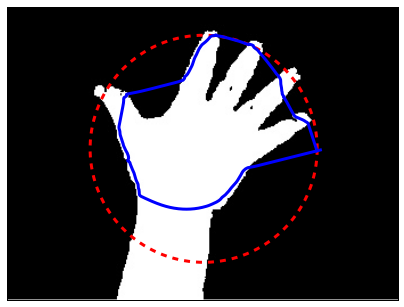
\includegraphics[scale=0.2]{res1}
              \caption{Naive use of the Active Contour algorithm}
          \end{figure}

\section*{3. Algorithm}

\begin{enumerate}

\item \textbf{Hand detection}\\
Backprojection algorithm or YUV space color detection. 
We are currently testing which one is better in terms of precision and speed

\item \textbf{Noise filtering}\\
We must find a method to remove the unwanted detected elements

\item \textbf{Initialization of the snake} \\
The snake must be initialized close to the hand.

\item \textbf{Active contour detection} \\
The Active contour algorithm's parameters must be optimized. 

\end{enumerate}

\section*{4. Tools}

We chose python because we are familiar with the language and we have a lot of libraried at our disposal. We decided to use OpenCV to detect colors and run the backprojection or YUV color detection on the image, and Scikit-Image for its Active Contour function.\\

\textbf{Language:} Python\\

\textbf{Libraries:} OpenCV (Color detection), Scikit-Image (Active Contour)\\






\end{document}